% Commuting square for the numerical round trip in
% docs/source/examples/mm_numeric_round_trip.rst
%
% Reducing and solving may be done in either order.  Going right-then-down reduces
% the system and then solves it; going down-then-right solves the original system
% and then translates its solution.  Both reach the same reduced solution.
%
% Build:  pdflatex commuting_square.tex
% To SVG: pdftocairo -svg commuting_square.pdf commuting_square.svg
%
\documentclass[border=8pt]{standalone}
\usepackage{amsmath}
\usepackage{tikz}
\usetikzlibrary{arrows.meta}

\begin{document}
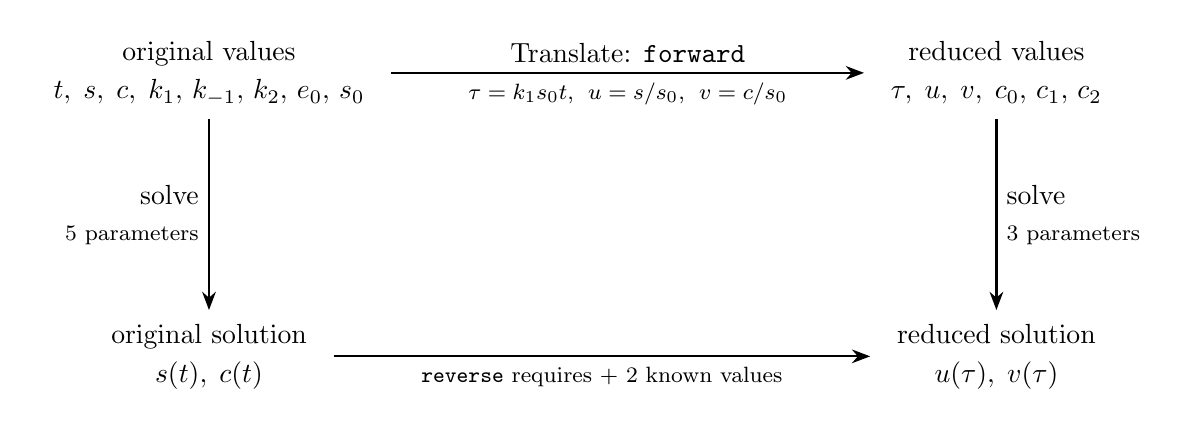
\begin{tikzpicture}[>=Stealth, thick]

  \node (NW) at (0, 0) {%
    \begin{tabular}{c}
      original values \\[2pt]
      $t,\; s,\; c,\; k_1,\, k_{-1},\, k_2,\, e_0,\, s_0$
    \end{tabular}};

  \node (NE) at (10, 0) {%
    \begin{tabular}{c}
      reduced values \\[2pt]
      $\tau,\; u,\; v,\; c_0,\, c_1,\, c_2$
    \end{tabular}};

  \node (SW) at (0, -3.6) {%
    \begin{tabular}{c}
      original solution \\[2pt]
      $s(t),\; c(t)$
    \end{tabular}};

  \node (SE) at (10, -3.6) {%
    \begin{tabular}{c}
      reduced solution \\[2pt]
      $u(\tau),\; v(\tau)$
    \end{tabular}};

  \draw[->] (NW) -- node[above]        {Translate: \texttt{forward}}
                  node[below, font=\footnotesize] {$\tau = k_1 s_0 t$,\; $u = s/s_0$,\; $v = c/s_0$}
            (NE);

  \draw[->] (SW) -- node[above]        {}
                  node[below, font=\footnotesize] {\texttt{reverse} requires $+$ 2 known values}
            (SE);

  \draw[->] (NW) -- node[left, align=right] {solve \\[1pt] {\footnotesize 5 parameters}} (SW);
  \draw[->] (NE) -- node[right, align=left] {solve \\[1pt] {\footnotesize 3 parameters}} (SE);

\end{tikzpicture}
\end{document}
